\documentclass[11pt,a4paper]{article}
\usepackage[latin1]{inputenc}
\usepackage[T1]{fontenc}
\usepackage{amsmath}
\usepackage{amsfonts}
\usepackage{amssymb}
\usepackage{graphicx}
\usepackage{here}
\usepackage{siunitx}
\usepackage{cleveref}
\usepackage{todonotes}

\author{Anders Brakestad, Luca Frediani, and Kathrin Helen Hopmann}
\title{Preliminary results: \\ BSSE-free association energies with MultiWavelets}
\begin{document}
	\maketitle
	\tableofcontents

\setcounter{secnumdepth}{1}

\section{Preface}
The aim of the project is to benchmark association reaction energies involving TM complexes with MRChem.
With a MW basis ``at'' the CBS limit, we automatically eliminate the BSSE, which is known to plague reaction energies.
We can therefore simplify the computational protocol by eliminating two birds with one stone: MW takes care of the BSIE problem related to GTO basis sets, and MWs also eliminate the need for carrying out annoying and complicated CP correction schemes.
The CP schemes are especially painful when trying to correct chemical transformation steps, in which case it is no longer obvious how to compute the BSSE.

Interesting questions:

\begin{enumerate}
	\item Is it OK to use a small basis set with CP correction, or is the BSIE too large?
			\todo[inline]{Anders: ``Normal'' GTO benchmarks should be capable of answering this. The BSIE of small GTO basis sets compared to large GTO basis sets, is likely much larger the the BSIE of large GTO basis sets compared to a high-precision MW basis.}
	\item Do MWs correct for both BSSE and BSIE? 
			\todo[inline]{Anders: I think yes, since in the limit of a complete basis both BSSE and BSIE go to zero.}
	\item Do precise MW corrections bring the reaction energy closer to the exact result?
			\todo[inline]{Anders: Based on preliminary results, this is not necessarily the case.}
\end{enumerate}

\section*{Computational details}
GTO calculations are run with ORCA version 4.2.1, and MW calculations are run with MRChem.

MW calculations performed with $\epsilon_{\text{rel}} = \num{1e-6}$

Several basis sets are currently tested: \verb|def2-svp|, \verb|def2-tzvp|, \verb|def2-qzvpp|, \verb|6-311g(d,p)|, and \verb|6-311+g(d,p)|.
Two functionals are currently being tested: \verb|bp86| and \verb|pbe0|.

Geometries are optimized with the \verb|def2-svp| basis set, with the following ORCA keyword line:

\begin{quote}
	\verb|! rks| \\
	\verb|! tightopt freq d3| \\
	\verb|! <functional> def2-svp grid5 finalgrid6| \\ 
	\verb|! rijcosx autoaux gridx5|
\end{quote}

Large-basis single-point calculations use the following keywords:

\begin{quote}
	\verb|! rks| \\
	\verb|! <functional> <basis_set> grid5 finalgrid6 d3 tightscf|
\end{quote}

The BSSE is estimated by Boys' and Bernardi's counterpoise correction, with the BSSE given by

\begin{equation} \label{eq: bsse}
\text{BSSE} = \Big(\Delta E^{\text{A}}_{\text{(A)}} - \Delta E^{\text{A}}_{\text{(AB)}} \Big) + \Big( \Delta E^{\text{B}}_{\text{(B)}} - \Delta E^{\text{B}}_{\text{(AB)}}\Big )			
\end{equation}

where the superscript indicates the molecular geometry and the subscript indicates the basis set.
This equation is easily derived from the following argument.
If the uncorrected and CP-corrected reaction energies are

\begin{align} \label{eq: rxn uncorrected}
\Delta E &= E^{\text{AB}}_{\text{(AB)}} - E^{\text{A}}_{\text{(A)}} - E^{\text{B}}_{\text{(B)}} \\ \label{eq: rxn corrected}
\Delta E^{\text{CP}} &= E^{\text{AB}}_{\text{(AB)}} - E^{\text{A}}_{\text{(AB)}} - E^{\text{B}}_{\text{(AB)}}
\end{align}

then the error (\cref{eq: bsse}) is the difference between them.
The corrected reaction energy then becomes

\begin{equation} \label{eq: }
\Delta E^{\text{CP}} = \Delta E + \text{BSSE}
\end{equation}

\section{Reactions studied}

\section{Overview of BSSE for the reactions}
\Cref{fig: bsse overview} presents the BSSE for all basis sets and all reactions. 
Systems with larger BSSEs may be of special interest in the benchmark, since the impact of
the MRChem calculations may be larger.
The figure shows that the Ni complexes exhibit larger BSSEs than the Cr complexes with the same ligands.
A possible rationalization: Ni has more electrons than Cr, and thus more basis functions.
Further, the tetrahedral geometry may lead to a larger electron density close to the metal, and thus in the overlapping region with the associating ligand, and therefore more basis functions, than the for the octahedral geometry.

\begin{figure}[H]
	\centering
	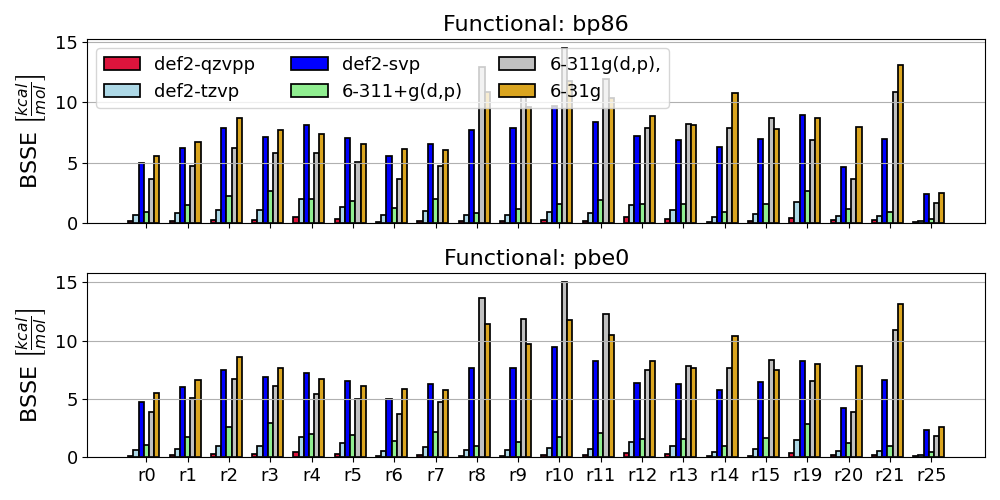
\includegraphics[width = \textwidth]{../figs/bsse.png}
	\caption{BSSEs for all BP86 (top) and PBE0 (bottom). Reactions 8--15 (Ni complexes) seem to have larger BSSEs than reactions 0--7 (Cr complexes).}
	\label{fig: bsse overview}
\end{figure}

\section{Overview of non-corrected association energies}

\section{Overview of CP-corrected association energies}

\end{document}